\documentclass[11pt]{article}

\usepackage{hyperref}
\setlength{\oddsidemargin}{0pt}
\setlength{\topmargin}{0pt}
\setlength{\textheight}{8.5in}
\setlength{\textwidth}{6.5in}
\usepackage{graphics}
\usepackage{graphicx}
\usepackage{color}
\usepackage{framed}

\begin{document}
\title{Seven-Letter Word\\Group 1 Final Report}

\author{
	Nipun Arora (nipun@cs.columbia.edu)
 \and Manuel Entrena Casas (mae2135@columbia.edu)
 \and Ben Warfield (bbw2108@columbia.edu)}

\date{December 14, 2009}
\maketitle
\begin{figure}
	\centering
	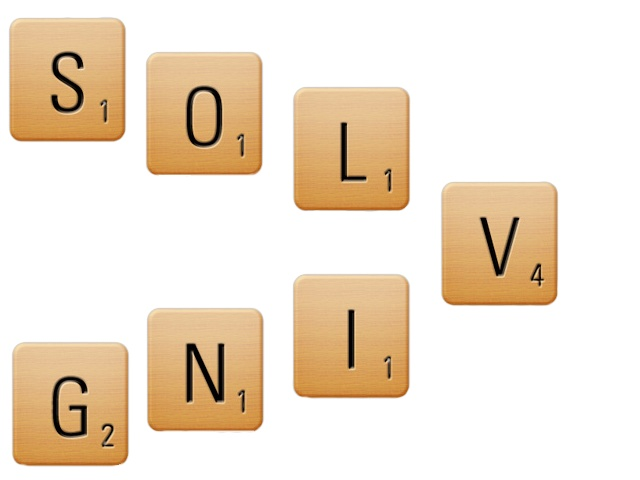
\includegraphics[width=0.7\textwidth]{cover}
\end{figure}


\newpage
\setcounter{tocdepth}{2}
\tableofcontents
\newpage

\section{ Introduction }

The aim of the project is to obtain a player that performs as well as possible in a modified version of Scrabble. In this version, the aim is still to form a word with the highest possible score from the letters that we have, but players must bid on the letters to get them, following the rules of the Vickrey auction.

\subsection{Word List}

For a word to be considered valid, it must be included in the provided dictionary. One of the challenges in the project will be searching words efficiently in this list. Therefore, the shorter we can make the list without altering the content, the faster our search for valid words will be. This is accomplished by:

\begin{enumerate}
\item removing words that cannot be formed with the set of letters in Scrabble
\item removing palindromes --words that contain the same letters but in different order
\end{enumerate}

\subsection{Maximizing Seven-Letter Words}

The reward for getting a seven-letter word is 50 points plus the score for each of the letters used in the word, whereas the score for a word with less than seven letters consists only of the sum of the individual letter scores. This means that forming a seven-letter word as often as possible is vital, since the difference in score is very big, and players will not be able to rely on non seven-letter words if they intend to win.

\subsection{Minimizing Costs}

Once it is clear that players must try to get seven-letter words, the next issue will be what cost we are willing to pay for the letters that allow us to form those words. The fact that we have to bid to get letters implies that we might end up forming a seven-letter word and still lose points if we are not careful while bidding so we do not bid more than we will get back. 

On the other hand, other players might use different strategies that force us to be more aggressive in our bidding strategy, so it will be important to balance the amount we bid according to the current situation, and static strategies will clearly be unsuccessful. 

\section{Framework}

There are two main tasks that our player must perform:

\begin{enumerate}
\item infer information from the current situation
\item decide the next action using that information
\end{enumerate}

The player framework that deals with the first task, including data structures and inference algorithms, is explained in the following section, while the tactics used to succeed in getting the necessary letters are explained in the Bidding Strategies section. 

\subsection{Player Architecture}

The basic concept our player architecture revolves around is that the more information we have, the better decisions we can make. Thus, we need to store many diverse facts so we can use that information to decide our next step. These include:

\begin{enumerate}
\item letters we currently have
\item letters that we assume are in the letter bag, thus considered obtainable
\item letters we know other players have
\item our current score and other players score
\item how much we have bid so far in the current round
\item how much all players have been bidding in the current round, as well as in past rounds
\item which words we can reach with the letters we have and the ones that are left in the bag
\item probability of reaching a word, based on the required letters for it
\end{enumerate}

\subsection{A Priori Algorithm} % BEN
\subsubsection{As originally designed}

Cite Agrawal '94.  Note originally implemented for COMS E6111.

\subsubsection{Modifications for Word Context}

Duplicate letters.  No, I'm not going to explain how I initially screwed it up, just how I eventually fixed it.

\subsection{Unreachable Words}

Each time a letter is picked up by another player, some words become impossible for our player to reach, no matter which tiles are available in the remaining auctions.  The data-mine structure (once letter repetition is allowed) actually provides a very easy way to find these words: any word that would require all the copies of this letter that are already in our rack, and all of the copies of this letter that were \textit{previously} in the letter bag, is now unreachable.  More explicitly, to find the newly-unreachable words, we must
\begin{enumerate}
\item find the number of copies of this letter that were in the letter bag before this tile was drawn (which may any where from 1 to 12)
\item find the number of copies of this letter that we have in our own rack
\item take the sum of these two numbers, and query the data mine for all words that include that number of this letter.
% that's kind of incoherent, Ben
\item if there are any such words, add them to our set of ``unreachable'' words.
\end{enumerate}

This technique will generally result in some words being marked as ``unreachable'' multiple times, but since the transition from reachable to unreachable is one-way, and the state maintenance is cheap (a simple array of booleans, indexed by word ID), the redundancy is of minimal concern.

\subsection{Probability Calculations} %BEN 

We can readily generate, at any time, the list of seven-letter words that we could reach this round.  However, at the beginning of a round, this list will contain both ``zymurgy'' and ``euchres,'' which are clearly not equally probable words for us to reach by the end of the round.

Obviously, we need some way to judge the relative ease of reaching each of the possible seven-letter words.  Ideally, this should be easy to recalculate as the letter distribution in the bag and on our rack shifts over the course of the round.

For a given configuration of the letter-bag and our own rack, we can calculate the number of possible draw sequences that would lead to a given word using fairly simple combinatorics--simple, at least, if we consider only draws that are relevant to the word itself.  For each a letter index $i$ between 1 (``A'') and 26 (``Z''), let $w_{i}$ be the number of appearances of that letter in a given word, $b_{i}$ be the number of copies of that letter remaining in the bag (or at least, potentially remaining there), and $r_{i}$ be the number of copies of that letter that we currently have on our rack.  Then the number of possible draw sequences that can lead to our being able to form this word is

% good thing we're not using Google, after all...
$$\prod_{i=1}^{26}{b_{i}\choose w_{i} - r_{i}}*\left( \sum_{i}w_{i} - r_{i}\right)!$$

Note that the factorial at the end for permutation is useless, since we're not actually doing the rest of the math, but it's useless at a constant rate for all the words that matter (seven-letter words will all have draw sequences of the same length, just differing likelihoods).

IF sum of $ \sum_{i}w_{i} - r_{i} > 7 - \sum_{i} r_{i}$ then $p = 0$ regardless (but this should already be excluded by the data-mining query).

caveat--hidden letters given to other players.  This doesn't change the possible draws, but it does change the number of rounds we have to try to get one of those draw sequences to happen.

Converting this to a concrete probability would involve a lot more math, but would iron out the problem of accounting for opportunity cost.  (Though not the problem of competition.)

\section{Bidding Strategies}

\subsection{When to Bid}

Our high-level bidding strategy is simple: we query the {\it a priori}-generated data mine using the set of letters we have in our rack at the moment, and determine what (if any) seven-letter words include them.  If any of these seven-letter words remains reachable (no matter how unlikely the possibility), we will bid only on letters that help us reach one of those words.
If no such word exists, we simply bid incrementally: we find the best-scoring word we can make with our existing rack and the best-scoring word we could make if we acquired the letter currently up for bid, then bid the difference (if positive) between the two scores.  This strategy, much discussed in class, has a worst-case behavior of zero gain, and (in contrast to any strategy that takes into account what other non-seven-letter words we might hypothetically form with other letters) is extremely simple to implement.

\subsection{Gain-based strategies}

Our initial approach to bidding (once we gave up on the ``bid 0 and make the best of it'' strategy) attempted to bid based on how much closer acquiring a particular letter would bring us to having a seven-letter word.  

This strategy is intuitively reasonable: if we succeed in every bid, we will have paid a cost no higher than the benefit (50 points) that we expect from forming a seven-letter word.

\subsubsection{Word Count}

Which we didn't actually implement, but is obvious to talk about.

\subsubsection{Summed Word Probabilities}

And ranked.

With replacement.

\subsubsection{Word Draw Possibilities}

The immediate problem here is that the possibilities count will virtually always go down when you acquire a new letter.  The best letters will reduce the count by only a small amount; the worst may reduce it to zero.

Cutoff-based bidding, still based on the tile value.

Cutoff-based bidding, based on Manuel's  % kind of optimistic ;-)
estimate of how much things were worth. 

\subsubsection{Summary}

These strategies successfully rescued our player from stinginess, allowing us to form seven-letter words with increasing frequency.  The cost they imposed, however, was disproportionate to the benefit: our player generally averaged significantly positive scores, but would fall far behind those of other groups.

\subsection{Loss-based strategies}

The obvious alternative to gain-based bidding is loss-based bidding: each time a letter is placed up for bid, we estimate how badly our chances of reaching a 7-letter word would be hurt by not acquiring it, then multiply that penalty by the benefit we would forgo (again, 50 points).  

\subsubsection{Basic Calculation}

Draw possibilities now - draw possibilities if this letter is removed from the bag.

\subsubsection{Opportunity Cost}

This strategy brings us back face to face with the problem we declined to solve earlier: how does the probability of a given sequence of letters being reached change with the number of remaining auctions?  

Our solution was sort of unsatisfactory, but our efforts to improve on it largely failed.

\subsubsection{Market Rates}

In principle, if we are able to form a perfect estimate of the opportunity cost of passing on one auction, as well as the penalty for failing to acquire each letter, we should be able to perfectly calculate the value (in expectation) of each letter, and our player should perform well, at least on average.  However, since our estimates are imperfect, and we may be in competition with other players, we also attempt to keep track of how our bids compare to the ``market rate'' for each letter: if we are losing out on our bids consistently, we may be systematically underestimating the value of letters.

We considered a number of tactics for adjusting our bidding to avoid falling behind on letter acquisition:

\begin{enumerate}
\item{} periodically boosting our bid by some fixed amount or factor, to avoid consistently being outbid (and confound any opposing-team predictors)
\item{} keeping track of the number of letters acquired and the number of bidding rounds, and boosting our bid if we are behind the ``average'' rate of letter acquisition (that is, if more than $1/7$ of letters have been auctioned off, but we have only 1 or 0 letters on our rack).
\item monitoring our success rate on recent bids, and boosting the bid by a fixed factor if we have been losing bidders some number of times in a row
\item extending the previous strategy by maintaining (or continuing to escalate) the boost factor until we succeed on a bid.
\item keeping track of the bidding statistics (average and standard deviation) to ensure that our bid is not too far from the average bid value, preventing under-bidding and over-bidding
\end{enumerate}

We evaluated all of these approaches in mini-tournaments, against each other and the most recent version of players from the other groups: our final conclusion was that the penalty for underbidding was not crippling us in any case, so a relatively conservative modification to our bidding would suffice.  Our final player tracks the success or failure of each non-zero bid, and boosts its bids by a factor of 2 if the last three or more non-zero bids have been unsuccessful.


\section{Tournament Results} % NIPUN
	Our G1Player seems to do pretty well in almost all tournaments, ranking amongst the top 2 teams on an average. We especially do well in tournaments with more opportunities to score seven letter words (i.e. more no of players). Overall we also seem to have formed the highest number of seven letter words out of all teams. On the other hand relative to other tournaments our performance in tournaments with lesser no of players is not as good. This basically clearly shows that given a good chance of forming seven letter words, we are generally the most successful amongst the given teams and do well in terms of the score. --Insert tables and graphs to illustrate above stuff
	
	Digging deeper into the tournament statistics we discovered that our success can basically be attributed to two factors:
	--Insert Graphs
	\begin{enumerate}
	\item{} A relatively high bid per letter: This is pretty obvious from the chart shown below, we definetely are amongst the top bidders per letter however we are not the highest.
	\item{} A good letter evaluation strategy
\end{enumerate}
	
	We also found that despite the fact that we are penalized heavily when we do not make seven letter words, this does not end up crippling our player as we more than make up for it with a high strike rate of forming seven letter words and a relatively high score gain when we form seven letter words.-- Illustrate with graphs
	
Special cases - One to one tournaments, all one player tournaments (do we want to speculate about the curious case of player 2 ) :P

\section{Issues Encountered/Observations/Lessons Learned}

Draw possibilities code had a bug early on which may have compromised some comparisons we made, but we are confident we ended up with a good solution.

\section{Possible Extensions}

Well, it might be interesting to have more explicit probability calculations for the late-game situation where you're trying to decide between a profitable increment and an unlikely seven-letter word.

You can't get an incredibly well-defined probability of getting what you need, but you can set an upper bound on it, which is all you need to see if the increment is worth more in expectation than trying for the 50-point bonus.  Very small enhancement, though.



\section{Acknowledgements}

Thanks for the acronym-eliminated word list, Jon.  Also the MySQL database for analysis purposes.

Also thanks to Professor Gravano for assigning the Agrawal paper and implementation for 6111.

And thanks to Dr. Virginia Warfield, Ph.D., for getting Ben interested in probability about 20 years ago.

\section{Contributions}



\section{Conclusion}
\end{document}
